%% LyX 2.1.4 created this file.  For more info, see http://www.lyx.org/.
%% Do not edit unless you really know what you are doing.
\documentclass[english]{article}
\usepackage[T1]{fontenc}
\usepackage[latin9]{inputenc}
\usepackage{graphicx}

\makeatletter
%%%%%%%%%%%%%%%%%%%%%%%%%%%%%% User specified LaTeX commands.
%% This document created by Scientific Word (R) Version 3.0




\usepackage{amsfonts}


%TCIDATA{OutputFilter=latex2.dll}
%TCIDATA{CSTFile=LaTeX article (bright).cst}
%TCIDATA{Created=Mon Nov 24 12:24:47 2003}
%TCIDATA{LastRevised=Fri Nov 28 11:39:52 2003}
%TCIDATA{<META NAME="GraphicsSave" CONTENT="32">}
%TCIDATA{<META NAME="DocumentShell" CONTENT="General\Blank Document">}
%TCIDATA{Language=American English}
\newtheorem{theorem}{Theorem}
\newtheorem{acknowledgement}[theorem]{Acknowledgement}
\newtheorem{algorithm}[theorem]{Algorithm}
\newtheorem{axiom}[theorem]{Axiom}
\newtheorem{case}[theorem]{Case}
\newtheorem{claim}[theorem]{Claim}
\newtheorem{conclusion}[theorem]{Conclusion}
\newtheorem{condition}[theorem]{Condition}
\newtheorem{conjecture}[theorem]{Conjecture}
\newtheorem{corollary}[theorem]{Corollary}
\newtheorem{criterion}[theorem]{Criterion}
\newtheorem{definition}[theorem]{Definition}
\newtheorem{example}[theorem]{Example}
\newtheorem{exercise}[theorem]{Exercise}
\newtheorem{lemma}[theorem]{Lemma}
\newtheorem{notation}[theorem]{Notation}
\newtheorem{problem}[theorem]{Problem}
\newtheorem{proposition}[theorem]{Proposition}
\newtheorem{remark}[theorem]{Remark}
\newtheorem{solution}[theorem]{Solution}
\newtheorem{summary}[theorem]{Summary}
\newenvironment{proof}[1][Proof]{\textbf{#1.} }{\ \rule{0.5em}{0.5em}}

\makeatother

\usepackage{babel}
\begin{document}

\title{Public Goods}


\author{Michael Peters}


\date{\today}

\maketitle

\section{Introduction}

In traditional economics, a public good is usually defined as something
that has two properties - non-excludability and non rivalrousness.
Non-rivalrousness means that if one person consumes a public good,
he or she doesn't take it away from anyone else. We don't need to
compete for public goods - they are there for all to consume. Non-excludability
means that it is impossible to prevent people from consuming the public
good once it is produced. Almost nothing fits the definition well
- maybe clean air. Some goods are non-excludable - a fireworks display,
loud music, but not obviously goods. Many public services are at least
potentially enjoyed by all, for example a bridge across a river, but
potentially subject to congestion.

Economists have long argued that government is needed to provide non-excludable,
non-rivalrous goods. Here is a really cute slide from Benjamin Allen
at Harvard University that sums up the argument.

\begin{center}
\includegraphics[scale=0.6]{Slide1}
\par\end{center}

In the figure, you can see the selfless cooperators working tirelessly
for no personal gain to make the world a better place. Evil free riders
take advantage of this selfless contribution of others and waste their
time in the pursuit of leisure (I guess that from the picture because
they are wearing baseball caps) which has no benefit to anyone but
themselves. The policy implication is that a public institution financed
by taxation is needed to force the free riders to pay. If nothing
else, this just makes things fairer for the cooperators.

Economic theory goes a bit further to argue that in the situation
described above too little of the public good will actually be provided.
The reason is that the selfless cooperators will actually stop producing
the public good at a point where the greedy free-riders would be willing
to pay them to produce more.

The point of this reading is two fold. First, to suggest why the story
above is misleading. Second, it explains why it is so important to
try to get this story right.

Public goods are often treated as a fringe element of microeconomic
theory - sometimes relegated to special topics courses. In fact, many
of the goods that are most important to us are at least non-rivalrous.
Modern technology makes most them non-excludable. The story above
suggests that it is those two properties - non-rivalrous and non-excludable
- are bad things that we need to try to get rid of just because they
are bad. In fact, they are the very properties that give goods value. 

A software program is an example, is something that is non-rivalrous
and non-excludable by nature. As in the picture above, it takes effort
to produce. If you run the same program as I do, I am not hurt by
that. The program is on a digital file, so it can be freely distributed
to everyone. Google, Facebook, Twitter are produce enormous amounts
of code that produce services that most of us seem to love. We can't
have evil free riders using that software to produce the same thing. 

Maybe you can see the problem with that argument. The first is that
all three companies seem to be free-riders. They use linux based tools
that are open source and free. According to a survey of the top 1
million websites in 2015 done by a tech analysis company called W3cook
(http://www.w3cook.com/), 98\% of the servers behind those websites
were using a Linux based (that is free) operating system. Your Wordpress
website is driven by open source software. The html and javascript
you use to make up your webpage are free open source software. At
least in the US, the power of the tech sector and silicon valley seems
to exist because software is non-rivalrous and non-exclusive. Those
are the properties that make the whole tech industry valuable.

Secondly, you might see that the simple distinction between cooperators
and free riders is completely wrong. The companies that support open
source software do it for their own benefit and produce software that
is useful to Google, etc. At the same time the software that Google
produces is offered back to the producers of the linux operating system.
The point being, that all of us are both cooperators and free-riders. 

The nice diagram given above, which perfectly summarizes what most
economists think about non-exclusiveness and non-rivalrousness, really
misses the point when it tries to describe things that are important
to us.

Perhaps a better way to describe a non-rivalrous good is to say that
it is a good that is produced at a possibly high fixed cost, but thereafter
has zero marginal cost. For software, one copy and a million copies
cost exactly the same thing. Music comes on mp3 files which can be
costlessly redistributed once they are produced. Researchers in universities
produce data and concepts that are useful to a lot of people. An idea
is non-rivalrous and non-excludable, as are jokes, fashion ideas,
newspaper articles, etc etc.

To understand the differences between all these examples, we can use
some of the basic ideas we have developed so far in consumer theory.
We'll use the old standby techniques 2 goods and two traders. One
good we'll just call money, denoted $x$, used for consuming other
stuff. The other good $y$ will be the one that is non-excludable
and non-rivalrous (in other words, produced at a cost, but they freely
available). We'll refer to $y$ as a public good from time to time.
Consumers have preferences $u\left(x,y\right)$ over these two goods
as they always do. Consumers can produce more of the public good by
giving up money.

The second idea is that since the public good $y$ is non-rivalrous,
if one consumer gives up money to produce more of the public good,
the other consumer will enjoy this new public good as well. This gives
us our selfless cooperator, and our selfish free rider. The difference
is that, as in real life, both consumers play both roles. Production
of the public good creates a very special type of positive externality
in the story that follows.

Now we can start with a description of something called the \emph{voluntary
contribution game}, which is a common way to think about how public
goods are provided. It explains why the amount of the public good
in the voluntary contribution game is too small (because the outcome
is not Pareto optimal: there is another outcome that will make both
consumers better off). 


\subsection{The voluntary contribution game}

Let $f\left(x\right)$ denote the amount of the public good that can
be produced from $x$ units of the private good. Suppose the two consumers
have utility functions $u_{1}\left(x,y\right)$ and $u_{2}\left(x,y\right)$
respectively. Their endowments of the private good are $\omega_{1}$
and $\omega_{2}$. The set of points $\left\{ \left(x,y\right):y=f\left(\omega_{1}+\omega_{2}-x\right)\right\} $
is the \emph{production possibilities frontier}. It looks exactly
like the production possibilities frontier that we studied before.

If the first consumer decides to consume $x_{1}$ (and devote the
rest of his endowment $\omega_{1}$ to production of the public good)
while consumer $2$ decides to consume $x_{2}$ the utilities of each
of the consumers are given by
\[
u_{1}\left(x_{1},f\left(\omega_{1}+\omega_{2}-x_{1}-x_{2}\right)\right)
\]
 for consumer $1$ and
\[
u_{2}\left(x_{2},f\left(\omega_{1}+\omega_{2}-x_{1}-x_{2}\right)\right)
\]
for consumer $2$. The important point is that if consumer $1$, say,
decides to consume a bit less of the private good and produce a bit
more of the public good, then consumer $2$ will enjoy the additional
public good too without any cost at all - that is what non-rivalrous
means.

At this point, we need to make some changes to what we have done before.
Each of the consumers simply picks the amount of the private good
they want on their own. This is a bit hard to do because the amount
that each consumer will choose to contribute depends on how much they
expect the other consumer to contribute. To handle this, we have to
replace \emph{Walrasian Equilibrium }with \emph{Nash equilibrium}.
Instead of taking prices to be fixed, each consumer takes the contribution
of the other consumer to be fixed and chooses the contribution that
maximizes his utility given this expectation. In the Nash equilibrium
each consumer must simultaneously choose his consumption of the private
good (analogously, his contribution to production of the public good)
while correctly forecasting what the other player will do.

Formally, a Nash equilibrium for the voluntary contribution game is
a pair of private consumptions $x_{1}^{\ast}$ and $x_{2}^{\ast}$
such that
\begin{equation}
u_{1}\left(x_{1}^{\ast},f\left(\omega_{1}+\omega_{2}-x_{1}^{\ast}-x_{2}^{\ast}\right)\right)\geq u_{1}\left(x^{\prime},f\left(\omega_{1}+\omega_{2}-x^{\prime}-x_{2}^{\ast}\right)\right)\label{consumer_1}
\end{equation}
 for any alternative contribution $x^{\prime}\in\left[0,\omega_{1}\right]$
and
\begin{equation}
u_{2}\left(x_{2}^{\ast},f\left(\omega_{1}+\omega_{2}-x_{1}^{\ast}-x_{2}^{\ast}\right)\right)\geq u_{2}\left(x^{\prime},f\left(\omega_{1}+\omega_{2}-x_{1}^{\ast}-x^{\prime}\right)\right)\label{consumer_2}
\end{equation}
 for any alternative contribution $x^{\prime}\in\left[0,\omega_{2}\right]$.

One way to view the outcome of this game is given in Figure $1$ where
the two consumers choose $x_{1}^{\ast}$ and $x_{2}^{\ast}$. The
`budget line' that consumer $1$ faces, for example, when consumer
$2$ chooses consumption $x_{2}^{\ast}$ is the set of all pairs $\left\{ \left(x_{1},y\right):y=f\left(\omega_{1}+\omega_{2}-x_{1}-x_{2}^{\ast}\right)\right\} $.
The slope of this is exactly the same as the slope of the production
possibilities frontier at the point $\left(x_{1}^{\ast}+x_{2}^{\ast},y^{\ast}\right)$.
The same is true for consumer $2$. So, in the equilibrium of the
voluntary contribution game, each consumer has the same marginal rate
of substitution and the same marginal rate of transformation in production.

\begin{center}
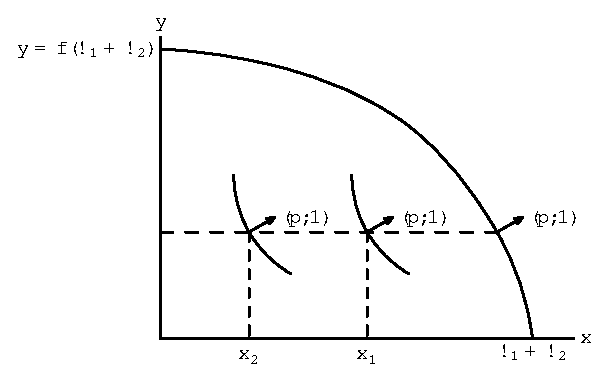
\includegraphics{public_goods_fig1}
\par\end{center}

With private goods, this is exactly what you want. Recall that, in
the Edgeworth box, both consumers' indifference curves were tangent
and the common slope of their indifference curves was equal to the
slope of the production possibilities frontier. With public goods,
this is not the outcome that you want.

You might be wondering what happened to the Edgeworth Box. Recall
that in the Edgeworth box, one point could be used to represent the
outcome for both consumers. The reason is that increasing the amount
of good $x$ that $1$ consumes automatically lowers the amount that
2 consumes. Good $x$ is rivalrous. In the usual story the same is
true of good $y$. Here, however, good $y$ is non-rivalrous - if
1 consumes more good $y$, then so does 2.

So lets modify the approach to account for this. For consumer 1, the
indifference curve is just the collection of $\left(x,y\right)$ pairs
that satisfy
\[
u_{1}\left(x,y\right)=K.
\]
The graphs of these curves look no different than they do in any other
problem. Higher indifference curves (further away from the origin)
represent higher values of $K$ in the equation above, and correspondingly
higher payoffs to consumers. 

The leap we are going to make here is that when we choose a bundle
$\left(x,y\right)$ for consumer 1, this bundle induces a corresponding
bundle for consumer 2 given by
\[
\left(\omega_{1}+\omega_{2}-f^{-1}\left(y\right)-x,y\right).
\]
In words, we figure out how much money is required to produce $y$,
that is the $f^{-1}\left(y\right)$, then subtract that from the total
endowment $\omega_{1}+\omega_{2}$ to get the total amount of money
left over after producing $y$ units of software. Subtract the $x$
we want to give to consumer 1, then give the rest to consumer 2. The
function $f^{-1}\left(y\right)$ is sometimes referred to as the cost
function for the public good.

Given this logic, we could define an indifference curve for \emph{consumer
2 }by finding all the consumption bundles for \emph{consumer 1 }that
induce the same payoff for player 2. Formally, an indifference curve
for player 2 is the collection of all bundles for player 1 that satisfy
\[
u_{2}\left(\omega_{1}+\omega_{2}-f^{-1}\left(y\right)-x,y\right)=K.
\]
\emph{ }

To figure out what these indifference curves look like is a bit daunting.
Holding $y$ constant, the less money consumer 1 has, the more is
left over for consumer 2. In this sense, player 2's indifference curves
represent higher payoffs for 2 the closer they are to the origin. 

For the rest, we'll rely on the idea that the public good provides
diminishing marginal utility to consumer 2. What that means is that
the more of the public good that is being produced, the less valuable
an additional unit of the public good will be. Fix the consumption
of the private good of consumer 1 at some value $x_{0}$ and travel
up the vertical line through $x_{0}$. Remember that changing the
public good in this case means that all the cost of producing the
public good is borne by consumer 2 since the amount of money consumer
1 has is being held constant at $x_{0}$. Initially as you increase
the public good, this makes consumer 2 better off since the public
good is very valuable to her when there isn't much of it. Eventually
the thrill will wear off, and as the production of the public good
gets higher and higher, consumer 2's payoff will begin to decline.
What that means is that consumer 2's indifference curves will typically
cross any vertical line twice.

Of course, there will be one indifference curve that is just tangent
to the vertical line. This one is illustrated in the picture below. 

In a Nash equilibrium, consumer 2 will choose how much of the public
good to produce assuming that the consumption of the public and private
good by consumer 1 are fixed. What that means is that consumer 2 will
choose a level of the public good at which her indifference curve
as we have just described it is vertical.

The indifference curves should look like backward C's as in the following
diagram, where I have superimposed consumer 2's indifference curve
into the original diagram depicting the Nash equilibrium of the voluntary
contribution game. Let me explain why. At the point where the indifference
curve is just tangent to the vertical line, consumer 2 could increase
her production of software $y$ and travel further up the vertical
line. If she travels directly upward, it means that she is holding
consumer 1's holdings of money constant. In other words, if she increases
production, she pays all the costs herself. At the tangency, she doesn't
want to do this - the marginal benefit she gets from increasing production
is exactly equal to the marginal cost. Formally
\[
\frac{\partial u_{2}\left(\omega_{1}+\omega_{2}-f^{-1}\left(y^{\ast}\right)-x_{1}^{\ast},y^{\ast}\right)}{\partial x}\frac{1}{f^{\prime}\left(y^{\ast}\right)}=\frac{\partial u_{2}\left(\omega_{1}+\omega_{2}-f^{-1}\left(y^{\ast}\right)-x_{1}^{\ast},y^{\ast}\right)}{\partial y}.
\]


Then if you travel up the vertical line a bit above $\left(x_{1}^{\ast},y^{\ast}\right)$,
then consumer 2 is strictly worse off. How to restore her payoff?
You have to give her more money, which means reducing the amount of
money you leave for consumer 1. That means that you have to travel
left of the vertical line to restore 2's payoff. The indifference
curve must lie to the left of the vertical line at every point except
at the tangency.

\begin{center}
\includegraphics{public_goods_fig5}
\par\end{center}

Since the point $\left(x_{1}^{\ast},y^{\ast}\right)$ is supposed
to coincide with the Nash equilibrium in the voluntary contribution
game, consumer 1's indifference curve has the same slope as the production
possibilities frontier at the point where $y^{\ast}$ is produced.
In other words, it is downward sloping, not vertical. The lens between
the curves represents a situation in which both consumers could be
made better off.

We draw the conclusion that the Nash equilibrium of the voluntary
contribution game is not pareto optimal. Remember what I have said
about 'pareto optimal' - it has nothing to do with optimal. An outcome
where consumer 2 gets whatever she likes, while consumer 1 gets nothing
is pareto optimal. Second, remember the lesson of Google, Facebook,
Twitter, all your social media products - they come from an equilibrium
that is not pareto optimal. It seems unlikely you would be too upset
about the products that are produced in that market, so maybe something
that isn't pareto optimal really isn't so bad.

Notice why it isn't so bad. All consumer are producers of the public
good - they are cooperators and free riders at the same time - they
help each other. Many important products have another property that
is relevant here. In the story above, if consumer 1 produces more
software, decreasing returns means that it is more expensive for consumer
2 to produce an \emph{extra }unit of software than it was before.
Software isn't like that, if consumer 1 produces more software, it
becomes cheaper for producer 2 to produce new software. If you let
me write more software, you will begin to want to write software that
was too hard or expensive to produce before. Music is also like that,
the more that is produced the easier it is to produce. Research is
like that, jokes are like that, newspaper articles are like that,
and many more. That probably explains why goods that are non-rivalrous
and non-exclusive are so often produced in such abundance - despite
the fact that the corresponding equilibrium outcome isn't pareto optimal. 

We won't develop this formally because we only have two goods, but
we can go much further. Benefiting from the efforts of another (what
we started out calling free riding) allows consumers to devote their
resources to other activities, these other activities may involve
production of public goods. Probably every organization on earth is
based on this principle. When one person volunteers to do some work
on something, the others in the organization don't free ride on this,
they use the time that has been freed to do other useful things. Most
organizations don't work perfectly, nonetheless many of them work. 


\section{Intellectual Property}

The reason it is so important to think about public goods and the
narrative of cooperators and free riders is because of the awful policies
it has spawned. The voluntary contribution game provides a sheen of
logic to a narrative which can then be easily misused. The outcome
in the voluntary contribution game is not pareto optimal, even though
it looks like all the other problems you encounter in intermediate
microeconomics. The reason appears to be that when a consumer produces
the public good, other people can use it. Other people can't use your
car because it is your property. Therefore we should turn public goods
into property - in other words, try to make a non-exclusive good into
an exclusive one. Then things would be pareto optimal again as they
are when all goods are private goods.

There are a bunch of laws that people now associate with intellectual
property - copyright law, trademarks and patents. They seem on the
surface to be associated with things that people thought up, so they
must be intellectual - therefore innovative. The story then goes that
we need laws to protect intellectual property to promote innovation.
There is a nice article by Richard Stallman at http://www.gnu.org/philosophy/not-ipr.en.html
which explains in a pretty simple way how these laws relate to one
another, and how none of them have anything to do with intellectual
property or promoting innovation.

You can read about US copyright and patent laws in a lovely (free)
book called ``Against Intellectual Monopoly'' by David Levine and
Michele Boldrin (http://www.dklevine.com/general/intellectual/againstfinal.htm).
The book is full of historical anecdotes and simple economic models
to explain what is going on. The gist of their argument is that copyright
and patent laws in the US are designed to give corporations levers
that they can use to prevent entry and suppress competition. Evidence
that these laws encourage creation of public goods is basically non-existent,
what evidence there is suggests the opposite. This is important for
Canada since the US almost always insists that countries adopt US
copyright and patent law before they will engage in trade negotiation.

So lets continue with the example of software patents, and try to
explain the effect that they have using our second year economic theory.

The way patents work is that one of the two consumers applies for
a patent, and is then given a monopoly over production of the patented
product, in this case our software. For example, Mircosoft has a couple
of strange patents - one is a patent for double clicking on an icon
to launch an application, awarded in 2004. Another is patent for using
the page up and page down buttons on a keyboard to shift the content
of a page up or down (2008). These operations are basic to just about
all software. Consistent with the patent, anyone writing software
would then have to pay microsoft a fee to use those procedures in
their software. 

You can see from these two examples, that patents (at least software
patents) have nothing to do with innovation. In Microsoft's defense,
they do need a portfolio of patents that they can use to defend themselves
against other large companies who also hold patents - often for no
better reason that to litigate a competitor out of existence (see
Apple's litigation against other smartphone makers https://en.wikipedia.org/wiki/Apple\_Inc.\_v.\_Samsung\_Electronics\_Co).

To make things simple here, we'll just assume that people have to
pay microsoft to produce their software for them. That really isn't
any different than having them pay a fee to microsoft whenever they
write their own software.

It might seem strange that microsoft could get a patent for a technique
people have been using forever. It is important to realize that the
US (and now Canada) has what is called a 'First to Patent' law, which
means that whoever files a patent on something first gets the patent
whether they developed the idea or not. 

Lets just assume that consumer 2 wins this race. Consumer 2 now owns
the public good. She can \emph{exclude }consumer 1 and charge whatever
price she likes for access to it. Suppose she sets the price $p$
for the public good.

Normally we do all our stuff using the price of good $x$ and letting
the price of good 1 be normalized to 1. We'll switch that here, but
this shouldn't create too much of a problem. The public good $y$
has a price $p$ , while the private good has price 1. Given the price
set by consumer 2, consumer 1 now finds the best bundle of public
and private goods he can afford. This is given by the point where
his indifference curve is tangent to the budget line that passes through
the point $\left(\omega_{1},0\right)$. Why care? The reason is that
consumer 1 will no longer be able to produce the public good on his
own (of if he does, he will have to pay consumer 2 a fee because she
owns the public good). So the price that consumer 2 sets will change
consumer 1's desire to have the public good. If consumer 2 sets a
price too high, consumer 1 won't want any.

What this means is that the patent doesn't by itself give consumer
2 any incentive to produce more of the public good - production depends
on price, which is chosen by consumer 2. What the patent does give
her is a device that she can use to extract money from consumer 1.

The figure below depicts what consumer 1 would want for three different
prices.

\begin{center}
\includegraphics{public_goods_fig6}
\par\end{center}

The steepest budget line is the one that has the lowest price for
the public good, the flattest budget line has the highest price. Since
2 now has the 'intellectual' monopoly, she can set any price that
she likes. She will pick the price that maximizes her payoff. 

It would seem quite daunting to find this price, since the change
in price will change consumer 1's consumption of the public good,
which will in turn effect how much consumer 2 needs to produce. 

Fortunately we have just the graphic device we need figure out what
consumer 2 will do, since we just figured out what her indifference
curves looked like in the space depicting consumer 1's consumption
of the private and public good. She will pick the price that put her
on the highest indifference curve consistent with consumer 1 maximizing
subject to his budget constraint. You'll notice in the curve above
that there is a smooth line that connects all the tangency points
for different prices. This curve is sometimes referred to as the offer
curve. The picture that follows shows what happens when consumer 2
chooses the point on this offer curve that is tangent to her own indifference
curve.

\begin{center}
\includegraphics{public_goods_fig7}
\par\end{center}

The indifference curve for consumer 2 is now tangent to consumer 1's
offer curve so consumer 2 is getting the best payoff she can get.
Consumer 1 is getting the best payoff he can afford. Notice that because
of the way the offer curve is drawn the two consumers indifference
curves won't be tangent. Both consumers would be better off if more
of the public good were produced. So the patent solution just produces
another inefficient outcome. This is why proponents of patents will
never talk about how well patents work. Instead they focus on how
bad the outcome is likely to be without them - we went over that -
not really so bad.

We can continue with graphic reasoning a bit more, but then we'll
need to switch to algebra. The following figure reproduces the outcome
for consumer 1 in the equilibrium of the voluntary contribution game.

\begin{center}
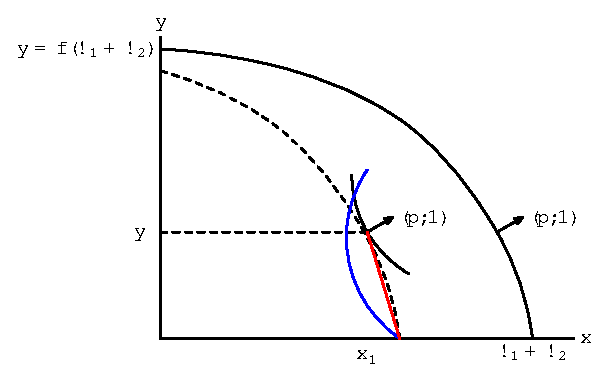
\includegraphics{public_goods_fig9}
\par\end{center}

Recall that the budget line for consumer 1 with patents starts at
his or her endowment point $\left(0,\omega_{1}\right)$. If consumer
2 sets a price for software which allows consumer 1 to buy the outcome
he enjoyed in the voluntary contribution game, then the budget line
consumer 1 faces would be given by the red line in the picture. Since
this budget line always lies below the production possibilities curve
that consumer 1 faces in the voluntary contribution game, it will
be steeper than consumer 1's indifference curve at his allocation
in the equilibrium of that game.

So far, this is completely working. If the price of the software were
set so that consumer 1 could reproduce the outcome in the voluntary
contribution game, then consumer 1 would be able to purchase the additional
software that he wants from consumer 2. Consumer 2 would in turn be
willing to produce it because she is making more than enough money
to compensate her for her additional cost.

What patents get wrong is what they do next - they give consumer 2
control over price. Most economics students understand at some level
that markets don't work when some market participant can control the
price. In this example, it is easy to see why this is the case. The
patent holder now has a new device for earning money that has nothing
at all to do with having to produce software. It would first occur
to her than since she controls price, she can actually get the same
level of the public good $y^{\ast}$ as in the voluntary contribution
game, while ending up with a lot more money for herself. 

In our formalism, we can use consumer 1's offer curve to understand
this. Since the budget line that consumer 1 faces when the price is
set in such a way that he can choose the equilibrium outcome in the
voluntary contribution game is steeper than his indifference curve
at that point, it means that consumer 1's offer curve cuts the horizontal
line through $y^{\ast}$ at a point to the left of consumer 1's original
equilibrium allocation. The offer curve should look like the solid
blue line in the figure above. So consumer 2 can raise the price of
software until the budget line faced by consumer 1 looks like the
green line in the next figure.

\begin{center}
\includegraphics{public_goods_fig10}
\par\end{center}

If you recall that the definition of the offer curve is all the points
at which consumer 1's indifference curve is tangent to a line that
runs from that point back to the endowment point, consumer 1 will
voluntarily choose $y^{\ast}$ units of software when the price is
set to the green line is the budget line. By allowing consumer to
control of the price, the patent basically creates a subsidy to the
patent holder. 

Consumer 2 might not be satisfied with this subsidy. She has really
embarked at this point on a new venture - surplus extraction. Software
is somewhat secondary at this point and she receives her reward by
manipulating price. It is theoretically possible that she might want
to raise output of software, but as in the figures above, this isn't
her main objective, it is to find the place where her indifference
curve is tangent to consumer 1's indifference curve.

Whether she does or not can be determined by traveling along the dashed
horizontal line to the left of the equilibrium point in the voluntary
contribution game until you reach the offer curve, given by the solid
blue line in the figure above. Since consumer 2 can achieve any point
on the offer curve that she wants, what she does will depend on what
her indifference curve looks like through that point. Generally, the
tangency with the offer curve may involve either more or less software
than in the voluntary contribution game. So patents are as likely
from a theoretical perspective to lower output of software as they
are to raise it.

Whether software patents work well or not is not a theoretical issue
- it all depends on preferences and costs. You might think that this
means that theory has nothing to say about whether patents are good
or bad. Yet the message of the theory is unambiguous - having a blanket
policy where everything is patented (or otherwise protected as 'intellectual
property') is going to do a lot of harm. 

We can illustrate this with a couple of familiar examples. We'll start
with one where patents act exclusively as a tax who proceeds are transferred
to the patent holder, then follow up with an example in which patents
can be beneficial to everyone (but more often than not just act as
a way of transferring income to patent holders). In each case we'll
follow the assumptions above, but assume that each consumer has money
income $\omega$ to begin. We'll also assume that each unit of software
can be produced for one unit of income. You should work out for yourself
what implications those assumptions have for the diagrams above. All
we'll change in the following two examples are consumer preferences.


\subsection*{Quasi-linear preferences}

Assume that consumer preferences are given by $u\left(x,y\right)=x+\ln\left(y\right)$,
where as above $x$ is money income, $y$ is software. In words preferences
are quasi-linear in income, a very common assumption in economics.
In the voluntary contribution game, each consumer's best reply is
determined by maximizing 
\[
x+\ln\left(2\omega-x-x_{2}\right)
\]
 where $x_{2}$ is the amount of money the other player retains for
herself. The solution is given by solving
\[
1=\frac{1}{2\omega-x-x_{2}},
\]
 so in the symmetric equilibrium of the voluntary contribution game
\[
x=\omega-\frac{1}{2}.
\]
This gives output of software in the voluntary contribution game as
$1$.

If consumer 2 is given a patent and sets the price $p$ for software,
consumer 1 will maximize
\[
\omega-py+\ln\left(y\right)
\]
 which, as you know, has solution $y=\frac{1}{p}$. We can write consumer
2's payoff for any price $p$ as
\[
\omega-\frac{1}{p}+1+\ln\left(\frac{1}{p}\right).
\]
Consumer 2 starts with $\omega$, but has to produce $\frac{1}{p}$
units of software as requested by consumer 1. This costs $\frac{1}{p}$.
She then receives $p$ times $\frac{1}{p}$ dollars of revenue from
consumer 1, which gives her $\omega-\frac{1}{p}+1$ dollars for herself,
and $\frac{1}{p}$ units of software. It is straightforward that consumer
2 will choose the price $p=1$, so that the same amount of software
is produced with patents as is produced in the voluntary contribution
game. 

What changes in the solution with patents is the distribution of income.
Consumer 2 ends up with payoff $\omega+\ln\left(1\right)=\omega$
while consumer 1 ends up with $\omega-1$. In other words, the patent
simply allows player 2 to charge player 1 for all the software, whereas
in the voluntary contribution game they would have split the cost.


\subsection*{Cobb-Douglas preferences }

Things work a bit better for patents when consumers have Cobb-Douglas
preferences. Under the right conditions, they can actually benefit
both consumers, though, for the most part, their main role is still
as a redistribution device. When preferences are Cobb-Douglas we have
\[
u\left(x,y\right)=x^{\alpha}y^{1-\alpha}.
\]
Consumer $1$ maximizes
\[
x^{\alpha}\left(2\omega-x-x_{2}\right)^{1-\alpha}
\]
where $x_{2}$ is the amount of income consumer 1 expects consumer
2 to retain for herself (which makes her contribution to the production
of software $\omega-x_{2}$). This is done subject to the constraint
that $x\le\omega$. 

The first order condition gives
\[
x=\alpha\left(2\omega-x_{2}\right)
\]
which has a solution between $0$ and $\omega$ provided $2\alpha$
is less than 1 and $x_{2}<\omega$. The symmetric equilibrium for
the voluntary contribution game is then 
\[
x=\frac{2\alpha}{1+\alpha}\omega
\]
 for each of the two players. The total output of software would then
be
\begin{equation}
2\omega-\frac{4\alpha}{1+\alpha}\omega=2\omega\frac{\left(1-\alpha\right)}{1+\alpha}.\label{voluntary-y}
\end{equation}


On the other hand, if 2 has the patent, then as you know, consumer
1 will keep the fraction $\alpha$ of his money income and choose
to buy $\frac{\left(1-\alpha\right)\omega}{p}$ units of the public
good. Since $\frac{2}{1+\alpha}\alpha\omega$ is obviously strictly
larger than $\alpha\omega$ you can see that consumer 1 will have
a lot less income with patents. 

So when 2 charges $p$ for the public good, her payoff is
\[
\left(\omega\left(2-\alpha\right)-\frac{\left(1-\alpha\right)\omega}{p}\right)^{\alpha}\left(\frac{\left(1-\alpha\right)\omega}{p}\right)^{\left(1-\alpha\right)}.
\]
To figure out whether 1 will end up with more of the public good,
we have to figure out what price 2 will choose. The price that maximizes
the expression above will also maximize
\[
\alpha\ln\left(\omega\left(2-\alpha\right)-\frac{\left(1-\alpha\right)\omega}{p}\right)+\left(1-\alpha\right)\ln\left(\frac{\left(1-\alpha\right)\omega}{p}\right)
\]
which is a little simpler. Differentiate it to get
\[
\frac{\alpha}{\omega\left(2-\alpha\right)-\frac{\left(1-\alpha\right)\omega}{p}}\frac{\left(1-\alpha\right)\omega}{p^{2}}-\frac{1-\alpha}{p}.
\]
This means that the price 2 will set satisfies
\[
\alpha\omega=p\left(\omega\left(2-\alpha\right)-\frac{\left(1-\alpha\right)\omega}{p}\right).
\]
This has solution. 
\[
p=\frac{1}{2-\alpha}.
\]


Now we can compare the two outcomes. Since consumer 1 determines the
output of software, the total amount of software produced with be
\[
\frac{\left(1-\alpha\right)\omega}{p}=
\]
Now lets use the diagram above to figure out whether 2 will want more
of less software than is created in the voluntary contribution game.
We can decompose her price adjustment into two parts. The first thing
we could imagine is that she takes the subsidy and raises the price
to the point where 1 will want the same level of the public good as
he did in the equilibrium of the voluntary contribution game. With
Cobb-Douglas preferences, the consumer will always want to keep $\alpha\omega$
of his income. So we want to find a price that make consumer 1 purchase
the level of output in the voluntary contribution game. From (\ref{voluntary-y})
this is $2\omega\frac{\left(1-\alpha\right)}{1+\alpha}$. So we want
a price such that 
\[
2\omega\frac{\left(1-\alpha\right)}{1+\alpha}=\frac{\left(1-\alpha\right)\omega}{p}
\]
or
\[
p=\frac{1+\alpha}{2}.
\]
It isn't too hard to show that $\frac{1+\alpha}{2}>\frac{1}{2-\alpha}$
for all $0<\alpha<1$, so consumer 2 will set a lower price for software
than the price that would have supported the same output of software
as in the voluntary contribution game.

We could have figured this out more directly. Once consumer 2 gets
a patent, she automatically receives a transfer of income from consumer
1. However, the size of the transfer doesn't change as 2 varies the
price because of the properties of Cobb Douglas preferences. So if
consumer 1 has Cobb Douglas preferences, the only way consumer 2 can
increase her payoff is by using the transfer to pay for more software
for herself.

More generally, if the consumer has more reasonable preferences for
which the proportion of income that she spends on software rises as
software prices rise, then consumer 2 will be able to extract even
more income from consumer 1 by raising software prices.

The fact that consumer 2 produces more software looks good, but it
doesn't mean that consumer 1 is any better off than she would have
been without the patent. 

If consumer 2 has the patent, then consumer 1 has payoff
\[
\left(\alpha\omega\right)^{\alpha}\left(\omega\left(1-\alpha\right)\left(2-\alpha\right)\right)^{1-\alpha}=
\]
\[
\omega\left(2-\alpha\right)\left(\frac{1}{2-\alpha}\right)^{\alpha}\left(\frac{\alpha}{\left(1-\alpha\right)}\right)^{\alpha}\left(1-\alpha\right).
\]
In the voluntary contribution game, consumer 1 has payoff 
\[
\left(\frac{2\alpha\omega}{1+\alpha}\right)^{\alpha}\left(2\omega\frac{1-\alpha}{1+\alpha}\right)^{1-\alpha}=
\]
\[
\frac{2}{1+\alpha}\omega\left(\frac{\alpha}{1-\alpha}\right)^{\alpha}\left(1-\alpha\right)
\]
To compare the payoffs, we need to compare $\omega\left(2-\alpha\right)\left(\frac{1}{2-\alpha}\right)^{\alpha}$
and $\frac{2}{1+\alpha}\omega$. We can't really figure this out analytically,
so we'll turn to the computer.

The next picture shows a plot of the payoffs of consumer 1 as they
vary with his propensity for keeping is own income, $\alpha$, when
$\omega=2$. This calculation, and the draft are drawn using wxMaxima,
which is a free computer algebra program. If you want to try it for
yourself, I left the code for the calculation at the top of the diagram.

Recall, that with CD preferences, $\alpha$ is the weight that the
consumer gives to retained income $x$ - if $\alpha$ is small, the
consumer desperately wants software and is willing to pay a lot for
it. If $\alpha$ is large, the consumer isn't so interested in software.
This is consistent with the \emph{demand }for software $\frac{1-\alpha}{p}$
- at any price, the consumer will buy less software the larger is
$\alpha$. The red curve in the figure below represents the function
$\frac{2}{1+\alpha}\omega$ which is the factor associated with the
equilibrium of the voluntary contribution game. The blue figure represents
the value of the factor associated with patents. The implication of
the fact that the red curve lies above the blue curve is that consumer
1 is never better off than he was in the equilibrium of the voluntary
contribution game. He gets more software, but the price of the software
is much more expensive to him than the software he would have produced
on his own. 

\[
\left(\alpha\omega\right)^{\alpha}\left(\frac{\left(1-\alpha\right)\omega}{p}\right)=\left(\alpha\omega\right)^{\alpha}\left(\frac{2\left(1-\alpha\right)\omega}{1+\alpha}\right)^{\left(1-\alpha\right)}
\]


\begin{center}
\includegraphics[scale=0.4]{maxima_plot}
\par\end{center}

We conclude that though the patent does result in more software being
produced, its primary purpose is still to transfer income to the patent
holder - essentially a tax.


\subsection*{Problems to work on.}

One way in which the model describe above differs from open source
software is that, with software, public good production tends to involve
increasing returns - the more software other people write, the more
software you can write for the same amount of money. Try to carry
out the analysis in the section with quasi-linear software above when
the production function for public goods is given by 
\[
y=x^{2}
\]
 where $y$ is output of the public good and $x$ is money spent on
developing the public good. Go as far as you can, but at the very
least, verify for yourself that when production is subject to increasing
returns, a lot more software will be produced in the voluntary contribution
game.
\end{document}
